\documentclass[letterpaper, conference]{IEEEtran}
\usepackage[left=1.62cm,right=1.62cm,top=1.9cm]{geometry}
\def\BibTeX{{\rm B\kern-.05em{\sc i\kern-.025em b}\kern-.08em
T\kern-.1667em\lower.7ex\hbox{E}\kern-.125emX}}
\IEEEsettopmargin{t}{2cm}
\setlength{\columnsep}{0.24in}
\usepackage{multirow}
\usepackage{enumitem}
\usepackage{tabularx,ragged2e,booktabs,caption}
\captionsetup{format=plain, labelfont={bf,footnotesize}, textfont=footnotesize}
\usepackage{subcaption}
\usepackage{array}
\usepackage{graphicx}
\usepackage{amsmath}
\usepackage{cite}
\interdisplaylinepenalty=2500
\usepackage{mathtools}
\usepackage{amsfonts}
\usepackage{amssymb}
\IEEEoverridecommandlockouts
\usepackage{balance}
\usepackage{float}
\usepackage{algorithm}
\usepackage{algpseudocode}
\usepackage{tikz}
\usetikzlibrary{arrows.meta, positioning, calc}
\algrenewcommand\alglinenumber[1]{\scriptsize #1:}
\renewcommand{\algorithmiccomment}[1]{\bgroup\hfill\it\scriptsize//~#1\egroup}
\newcolumntype{P}[1]{>{\centering\arraybackslash}p{#1}}

\begin{document}
\addtolength{\tabcolsep}{-6pt}
\DeclareGraphicsExtensions{.pdf,.png,.gif,.jpg}

\title{UTSON: A Topology-Aware Signal Control Framework for Urban Traffic}

\author{\IEEEauthorblockN{Dhairya Rupani,\textsuperscript{*} Drumil Bhati,\textsuperscript{*} and Abhishek Chakraborty}
\IEEEauthorblockA{School of Engineering and Applied Science, Ahmedabad University, Ahmedabad, Gujarat 380009, India\\
dhairya.r@ahduni.edu.in,\ drumil.b@ahduni.edu.in,\ abhishek2003slg@ieee.org}
\thanks{\textsuperscript{*}The authors contributed equally to this work.}}

\maketitle

\begin{abstract}
Urban congestion worsens when fixed-time signal plans cannot respond to stochastic demand. We present the Urban Traffic Signal Optimization Network (UTSON), a topology-aware, discrete-time signal control framework that minimizes cumulative waiting time by integrating the global road network into decentralized intersection decisions. UTSON evaluates three control policies (Fixed-Time, Backpressure, and the proposed Waiting-Time Minimization (WTM) controller) across four cities from OpenStreetMap: Bengaluru, Berlin, London, and Sydney. The WTM controller combines multiplicative hub-awareness with dynamic parameter scaling, achieving up to 198.0\% throughput improvement (over Backpressure) and 26.6\% travel-time reduction (over Fixed-Time), while remaining fully interpretable and requiring no training data.
\end{abstract}

\begin{IEEEkeywords}
Urban traffic control, betweenness centrality, adaptive signal timing, waiting time minimization, discrete-time simulation, complex network analysis.
\end{IEEEkeywords}

%%=============================================================
\section{Introduction}
\label{section_Introduction}
%%=============================================================
\IEEEPARstart{S}{ignalized} intersections are the primary bottlenecks of urban mobility. Congestion at a few critical nodes propagates upstream across an entire network within minutes, costing cities billions annually in lost productivity and excess emissions~\cite{ibe2013markov}. Most deployed systems rely on fixed-time plans calibrated to historical averages: simple to operate, but unable to react to stochastic, real-time demand. Adaptive extensions exist but respond only to the immediate local queue, ignoring the broader network structure and the fact that intersections lying on many shortest paths are inherently more prone to causing city-wide spillback when saturated.

A fundamental limitation of purely local controllers is that they treat every intersection as structurally equivalent. In reality, road networks are heterogeneous: a handful of high-betweenness nodes, such as bridge approaches and arterial merges, carry a disproportionate share of city-wide routing demand~\cite{newman2010networks}. When one of these nodes saturates, vehicles cannot enter the saturated link and queue on upstream edges, which in turn block their feeder intersections, triggering a cascade that can immobilize large network segments within a few signal cycles~\cite{daganzo1994queue}. A controller that can identify these structurally critical nodes in advance and pre-allocate green time before queues reach critical length has a fundamentally better chance of containing congestion. This cascade-prevention property cannot be achieved by reactive controllers that observe only instantaneous local queues; it requires a global structural descriptor of the network.

Graph-theoretic analysis offers exactly such a descriptor. Betweenness centrality quantifies how often a node appears on shortest paths between all origin-destination pairs and is a proven predictor of structural importance in complex networks~\cite{freeman1977set, brandes2001centrality}. In transportation, nodes with high betweenness lie along dominant routing corridors; their saturation has the greatest network-wide impact. While centrality measures have been applied to offline road-network analysis~\cite{wang2015graph}, their integration into real-time signal control has remained largely unexplored. Adaptive controllers that do incorporate global graph structure typically rely on GNN-based representations~\cite{zhang2021trafficgcn}, which require large training datasets, high inference overhead, and produce black-box decisions that are difficult to certify for safety-critical infrastructure. A lightweight, analytically grounded mechanism for embedding betweenness centrality directly into a decentralized controller score has not previously been proposed.

In this paper, we address the following question: \emph{Can global topological awareness be integrated into decentralized signal control to preemptively mitigate congestion at structurally critical intersections before it cascades network-wide?} The major contributions of the paper are as follows:
\begin{enumerate}[label=(\roman*),leftmargin=*]
\item A lightweight, topology-aware \textbf{Waiting-Time Minimization (WTM)} controller that uses a multiplicative hub-awareness formulation and dynamic parameter scaling derived from local graph metrics, providing global awareness without centralized overhead.
\item A reproducible discrete-time simulation framework integrating real-world OpenStreetMap topologies with stochastic demand models for scalable policy benchmarking.
\item Cross-topology validation across four cities (Bengaluru, Berlin, London, Sydney) and an empirical comparison of four centrality measures, establishing betweenness centrality as the most robust structural prior for urban traffic control.
\end{enumerate}
The paper is structured as follows: Section~\ref{section_related} reviews related work, Section~\ref{section_preliminaries} establishes the mathematical foundations; Section~\ref{section_methodology} presents the UTSON framework; Section~\ref{section_exp_setup} describes the experimental setup; Sections~\ref{section_exp_res} and~\ref{section_discussion} present the experimental results, discussion, and analysis; Section~\ref{limit_and_fut_work} outlines the limitations and future work; and Section~\ref{section_conclusion} concludes the paper.


%%=============================================================
\section{Related Work}
\label{section_related}
%%=============================================================
Conventional signal controllers use time-constrained plans optimized on historical flows, but these cannot accommodate stochastic, dynamic demand~\cite{daganzo1994queue}. The literature has therefore developed along three broad tracks: pressure-based reactive methods, adaptive and learning-based methods, and graph-topology-aware methods.

\textbf{Pressure-based and backpressure methods.}
The theoretical foundation was established by Tassiulas and Ephremides~\cite{tassiulas1992stability}, who proved that max-weight scheduling stabilizes queues and maximizes throughput under any feasible demand in multihop networks. Varaiya~\cite{varaiya2013maxpressure} extended this to urban signalized intersections as max-pressure (MP) control, prioritizing phases based on the cross-link queue difference. MP provably stabilizes any network within its saturation envelope, but suffers from ``last-vehicle'' starvation: a near-empty queue can monopolize green time, starving competing approaches. Zaidi et al.~\cite{zaidi2016backpressure} coupled backpressure with adaptive vehicle re-routing to improve throughput, though their model requires that all vehicles can change routes dynamically. Li et al.~\cite{li2018delay} introduced delay-based extensions at isolated intersections, combining instantaneous queue pressure with accumulated waiting time to jointly optimize throughput and fairness. Across all these methods, the structural position of the intersection in the wider network plays no role: a bridge approach and a minor side road are treated identically if their instantaneous queues match.

\textbf{Adaptive and learning-based methods.}
Practical adaptive control began with systems such as SCATS~\cite{lowrie1982scats} and SCOOT~\cite{gartner2005state}, which adjust cycle lengths and green splits in real time based on loop-detector occupancy. These systems achieve measurable reductions in travel time but are fundamentally reactive: they respond to detected congestion rather than anticipating its likelihood. Neural network controllers~\cite{srinivasan2008network} improved responsiveness by learning nonlinear mappings from detector states to green-time decisions, though the resulting policies remain local and opaque. Single-agent RL applied to isolated intersection control~\cite{abdulhai2003reinforcement} showed that adaptive policies could be learned without an explicit traffic model; multi-agent RL~\cite{wiering2000multi} extended this to neighborhood-level coordination. Deep Q-networks with prioritized replay~\cite{liang2020contextual} improved sample efficiency but maintained a local coordination horizon. Coordinated centralized adaptive control~\cite{gartner2005state} extended the horizon to arterial corridors via green-band optimization yet depends on fixed detector infrastructure. GNNs combined with multi-agent RL~\cite{zhang2021trafficgcn} capture global spatio-temporal correlations but incur substantial training cost and produce black-box decisions difficult to audit for real-world deployment.

\textbf{Graph topology and centrality in traffic.}
Urban road networks have been studied as complex graphs to characterize congestion susceptibility~\cite{newman2010networks, wang2015graph}. Betweenness centrality~\cite{freeman1977set, brandes2001centrality} identifies nodes on many shortest paths that are first to saturate under demand; PageRank-style measures~\cite{pagerank2016centrality} rank intersections by influence but do not reflect path-level routing pressure directly. Despite this body of analysis, betweenness centrality has not been used as a live per-step scoring prior in any decentralized real-time controller.

\textbf{Positioning of UTSON.}
UTSON bridges structural network analysis and real-time decentralized control. Relative to backpressure methods, it weights each approach by the global importance of its source node, enabling cascade-preventive prioritization before queues form. Compared with GNN-based approaches, it requires no training data, has $\mathcal{O}(k(|E|+|V|\log|V|))$ pre-computation, and produces fully interpretable scores. In contrast to corridor controllers, it operates over the entire network graph. Table~\ref{tab:lit_review} maps this position.

\begin{table*}[t]
\centering
\caption{Summary of traffic signal control literature and identified gaps}
\label{tab:lit_review}
\renewcommand{\arraystretch}{1.3}
\begin{tabularx}{\textwidth}{|>{\raggedright\arraybackslash}p{2.6cm}|>{\raggedright\arraybackslash}X|>{\raggedright\arraybackslash}X|>{\raggedright\arraybackslash}X|>{\raggedright\arraybackslash}X|}
\hline
\textbf{Reference} & \textbf{Control Paradigm} & \textbf{Topology Awareness} & \textbf{Core Objective} & \textbf{Key Limitation} \\
\hline
Tassiulas et al.~\cite{tassiulas1992stability} & Max-weight backpressure & Link-level only & Queue stability \& throughput & No urban transit constraints \\
\hline
Varaiya~\cite{varaiya2013maxpressure} & Max-pressure & Upstream/downstream queues & Maximize throughput & Last-vehicle starvation \\
\hline
Zaidi et al.~\cite{zaidi2016backpressure} & Backpressure + adaptive routing & Localized dynamic pathing & Queue reduction \& routing & Requires full vehicle reroutability \\
\hline
Li et al.~\cite{li2018delay} & Delay-based queue reactive & Isolated intersection & Throughput + fairness & No global network foresight \\
\hline
Abdulhai et al.~\cite{abdulhai2003reinforcement} & Single-agent RL & None & Adaptive policies w/o models & No network-level coordination \\
\hline
Wiering~\cite{wiering2000multi} & Multi-agent RL & Neighborhood-level & Decentralized cooperation & No global structural awareness \\
\hline
Lowrie~\cite{lowrie1982scats} & SCATS (adaptive cycle) & None & Real-time cycle adjustment & Cannot anticipate network cascades \\
\hline
Srinivasan et al.~\cite{srinivasan2008network} & Neural network & None & Learned signal timing & Black-box; no topological reasoning \\
\hline
Liang et al.~\cite{liang2020contextual} & Deep Q-network & None & Efficient single-intersection control & No network-level coordination \\
\hline
Gartner~\cite{gartner2005state} & SCOOT / centralized arterial & Corridor-level & Arterial green-band optimization & Fixed infrastructure; no global graph \\
\hline
Zhang et al.~\cite{zhang2021trafficgcn} & GNN + coordinated RL & Global (GNN features) & Predictive congestion management & High overhead; black-box decisions \\
\hline
\textbf{UTSON (ours)} & Topology-aware WTM & Global betweenness centrality & Minimize wait; prevent cascades & Lightweight, interpretable, no training \\
\hline
\end{tabularx}
\end{table*}

%%=============================================================
\section{Preliminaries}
\label{section_preliminaries}
%%=============================================================

This section establishes the mathematical foundations and graph-theoretic concepts upon which the UTSON framework is built.

\subsection{Road Network and Edge Attributes}
The road network is modeled as a directed graph $G=(V,E)$~\cite{newman2010networks}, where nodes $v\in V$ are signalized intersections and directed edges $e=(u,v)\in E$ are one-way road segments. Attributes $L_e$ (length), $V_e$ (speed limit), and $\ell_e$ (lane count) are parsed from OpenStreetMap~\cite{boeing2017osmnx} via OSMnx. Only the largest strongly connected component is retained; parallel multi-edges are collapsed to the shortest. Free-flow travel time and per-cycle service capacity are:
\begin{equation}
\tau_e = \frac{L_e}{V_e}, \qquad
C_e = \max\!\left(1,\lfloor 8\ell_e\rfloor\right), \label{eq:tau_cap}
\end{equation}
where the constant $8$ follows the standard 1800~veh/hr/lane saturation flow assumption~\cite{hcm2016}, and $\max(\cdot,1)$ prevents division-by-zero on unmapped edges.

\subsection{Betweenness Centrality}
Node importance is quantified by weighted betweenness centrality~\cite{freeman1977set,brandes2001centrality}:
\begin{equation}
B_i = \sum_{s\neq i\neq t}\frac{\sigma_{st}(i)}{\sigma_{st}}, \qquad
\hat{B}_i = \frac{B_i}{\max_j B_j}\in[0,1], \label{eq:bc}
\end{equation}
where $\sigma_{st}$ is the number of $\tau_e$-weighted shortest paths from $s$ to $t$ and $\sigma_{st}(i)$ is those passing through $i$. High-$\hat{B}$ nodes lie on many shortest paths; their saturation can trigger network-wide congestion cascades. To keep computation tractable, $B_i$ is approximated by sampling $k{=}80$ source nodes, reducing complexity from $\mathcal{O}(|V||E|)$ to $\mathcal{O}(k(|E|+|V|\log|V|))$.

\subsection{Stochastic Demand and Signal Timing}
Vehicle arrivals follow a Poisson process~\cite{ross2014poisson,daganzo1994queue}: $A_t\sim\mathrm{Poisson}(\lambda)$, where $A_t$ is the number of vehicles injected at step $t$ and $\lambda$ is the mean arrival rate. Each vehicle is assigned a precomputed OD route directed through structural chokepoints. Rather than managing explicit stateful timers, UTSON uses a \emph{virtual green time} abstraction: a dynamic green duration $g_{\mathrm{dynamic}}\in[g_{\min},g_{\max}]$ is computed at each step proportional to the approach urgency and converted into a discrete vehicle discharge count (details in Section~\ref{subsec:edge_capacity}).

%%=============================================================
\section{UTSON Framework Design}
\label{section_methodology}
%%=============================================================

This section presents the UTSON framework: a discrete-time, topology-aware signal control system built on the foundations of Section~\ref{section_preliminaries}. We detail the three evaluated control policies, the multiplicative hub-awareness scoring mechanism, the dynamic topology scaling of control parameters, and the edge-level capacity allocation procedure. Fig.~\ref{fig:utson_block} presents the complete UTSON system architecture.

\begin{figure*}[t]
\centering
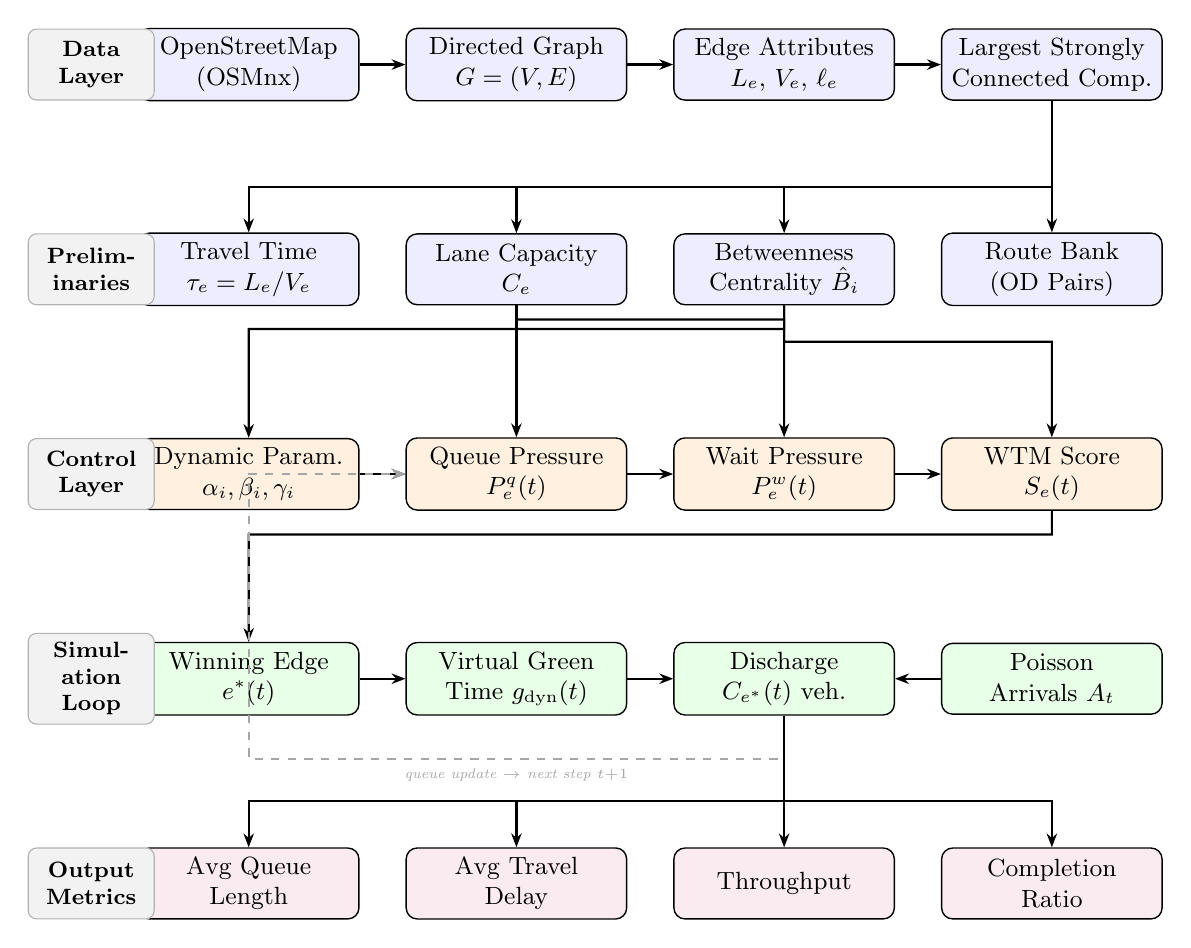
\begin{tikzpicture}[
  %% Node styles
  iblock/.style ={draw, rounded corners=4pt, minimum width=2.8cm, minimum height=0.9cm,
                  align=center, font=\small, fill=blue!7,  line width=0.5pt},
  cblock/.style ={draw, rounded corners=4pt, minimum width=2.8cm, minimum height=0.9cm,
                  align=center, font=\small, fill=orange!12, line width=0.5pt},
  sblock/.style ={draw, rounded corners=4pt, minimum width=2.8cm, minimum height=0.9cm,
                  align=center, font=\small, fill=green!9,  line width=0.5pt},
  oblock/.style ={draw, rounded corners=4pt, minimum width=2.8cm, minimum height=0.9cm,
                  align=center, font=\small, fill=purple!8, line width=0.5pt},
  %% Label strip on the left
  lstrip/.style ={draw=gray!60, fill=gray!10, rounded corners=3pt,
                  minimum width=1.6cm, align=center, font=\bfseries\footnotesize},
  %% Arrows
  arr/.style  ={-{Stealth[length=5pt]}, thick},
  darr/.style ={-{Stealth[length=5pt]}, thick, dashed, gray!70},
  %% Column x-positions (centres)
  /tikz/col1/.initial=1.8,
  /tikz/col2/.initial=5.2,
  /tikz/col3/.initial=8.6,
  /tikz/col4/.initial=12.0,
  %% Row y-positions (centres)
  /tikz/rowA/.initial= 0.0,    % Data Layer
  /tikz/rowB/.initial=-2.6,    % Preliminaries
  /tikz/rowC/.initial=-5.2,    % Control Layer
  /tikz/rowD/.initial=-7.8,    % Simulation Loop
  /tikz/rowE/.initial=-10.4    % Output Metrics
]

%% ── ROW A: DATA LAYER ─────────────────────────────────────────
\node[iblock] (osm)   at (1.8,  0.0) {OpenStreetMap\\(OSMnx)};
\node[iblock] (graph) at (5.2,  0.0) {Directed Graph\\$G=(V,E)$};
\node[iblock] (attrs) at (8.6,  0.0) {Edge Attributes\\$L_e,\,V_e,\,\ell_e$};
\node[iblock] (scc)   at (12.0, 0.0) {Largest Strongly\\Connected Comp.};

\draw[arr] (osm)   -- (graph);
\draw[arr] (graph) -- (attrs);
\draw[arr] (attrs) -- (scc);

\node[lstrip, minimum height=0.9cm] at (-0.2, 0.0) {Data\\Layer};

%% ── ROW B : PRELIMINARIES ───────────────────────────────────────
\node[iblock] (tau) at (1.8,  -2.6) {Travel Time\\$\tau_e = L_e/V_e$};
\node[iblock] (cap) at (5.2,  -2.6) {Lane Capacity\\$C_e$};
\node[iblock] (bc)  at (8.6,  -2.6) {Betweenness\\Centrality $\hat{B}_i$};
\node[iblock] (rte) at (12.0, -2.6) {Route Bank\\(OD Pairs)};

%% SCC fans out to all four prelim nodes — use a common drop point
\coordinate (sccDrop) at (12.0, -1.55);
\draw[arr] (scc.south) -- (sccDrop) -| (tau.north);
\draw[arr] (sccDrop)   -| (cap.north);
\draw[arr] (sccDrop)   -| (bc.north);
\draw[arr] (sccDrop)   -- (rte.north);

\node[lstrip, minimum height=0.9cm] at (-0.2, -2.6) {Prelim-\\inaries};

%% ── ROW C : CONTROL LAYER ───────────────────────────────────────
\node[cblock] (dyn)   at (1.8,  -5.2) {Dynamic Param.\\$\alpha_i,\beta_i,\gamma_i$};
\node[cblock] (pq)    at (5.2,  -5.2) {Queue Pressure\\$P_e^{q}(t)$};
\node[cblock] (pw)    at (8.6,  -5.2) {Wait Pressure\\$P_e^{w}(t)$};
\node[cblock] (score) at (12.0, -5.2) {WTM Score\\$S_e(t)$};

%% bc -> dyn  (diagonal avoided via explicit waypoint)
\draw[arr] (bc.south)  -- ++(0,-0.30) -- ++(-6.8,0) -- (dyn.north);
%% cap -> pq
\draw[arr] (cap.south) -- (pq.north);
%% cap -> pw  (offset to avoid overlap with cap->pq)
\draw[arr] (cap.south) -- ++(0,-0.18) -- ++(3.4,0) -- (pw.north);
%% bc  -> score
\draw[arr] (bc.south)  -- ++(0,-0.46) -- ++(3.4,0) -- (score.north);
%% dyn,pq,pw -> score  (horizontal within row)
\draw[arr] (dyn)   -- (pq);
\draw[arr] (pq)    -- (pw);
\draw[arr] (pw)    -- (score);

\node[lstrip, minimum height=0.9cm] at (-0.2, -5.2) {Control\\Layer};

%% ── ROW D : SIMULATION LOOP ─────────────────────────────────────
\node[sblock] (win)  at (1.8,  -7.8) {Winning Edge\\$e^*(t)$};
\node[sblock] (gt)   at (5.2,  -7.8) {Virtual Green\\Time $g_{\mathrm{dyn}}(t)$};
\node[sblock] (disc) at (8.6,  -7.8) {Discharge\\$C_{e^*}(t)$ veh.};
\node[sblock] (poi)  at (12.0, -7.8) {Poisson\\Arrivals $A_t$};

%% score -> win
\draw[arr] (score.south) -- ++(0,-0.30) -- ++(-10.2,0) -- (win.north);
%% within row
\draw[arr] (win)  -- (gt);
\draw[arr] (gt)   -- (disc);
%% poi feeds into disc from right
\draw[arr] (poi.west) -- (disc.east);
%% feedback: disc -> pq  (route along bottom, clear of all nodes)
\draw[darr] (disc.south) -- ++(0,-0.55)
    -- ++(-6.8,0)
    node[midway, below, font=\tiny\itshape] {queue update $\to$ next step $t{+}1$}
    |- (pq.west);

\node[lstrip, minimum height=0.9cm] at (-0.2, -7.8) {Simul-\\ation\\Loop};

%% ── ROW E : OUTPUT METRICS ──────────────────────────────────────
\node[oblock] (avq)  at (1.8,  -10.4) {Avg Queue\\Length};
\node[oblock] (avt)  at (5.2,  -10.4) {Avg Travel\\Delay};
\node[oblock] (tput) at (8.6,  -10.4) {Throughput};
\node[oblock] (comp) at (12.0, -10.4) {Completion\\Ratio};

%% disc fans out to all four output nodes
\coordinate (discDrop) at (8.6, -9.35);
\draw[arr] (disc.south) -- (discDrop) -| (avq.north);
\draw[arr] (discDrop)   -| (avt.north);
\draw[arr] (discDrop)   -- (tput.north);
\draw[arr] (discDrop)   -| (comp.north);

\node[lstrip, minimum height=0.9cm] at (-0.2, -10.4) {Output\\Metrics};

\end{tikzpicture}
\caption{UTSON system architecture. Raw OpenStreetMap data is parsed into a directed graph (Data Layer); graph metrics including travel time, capacity, betweenness centrality, and OD routes are precomputed (Preliminaries); node-specific scoring parameters and pressure signals are assembled (Control Layer); the WTM controller selects a winning edge, computes virtual green time, and discharges vehicles each step (Simulation Loop); performance metrics are recorded at every step (Output Metrics). The dashed feedback arrow shows that queue states updated during discharge feed back into the next step's pressure computations.}
\label{fig:utson_block}
\end{figure*}

UTSON evaluates three signal-control policies under identical simulation conditions, spanning a spectrum from static baseline to fully adaptive topology-aware control:
\begin{enumerate}[leftmargin=*]
\item \textbf{Fixed-time:} Equal cyclic allocation regardless of queue state (the real-world baseline).
\item \textbf{Backpressure (BP):} Prioritizes the approach with maximum instantaneous queue; local-reactive only.
\item \textbf{WTM (proposed):} Jointly considers queue pressure, cumulative waiting, and betweenness centrality for preemptive, topology-aware control.
\end{enumerate}

\subsection{Additive Baseline Score}
For edge $e$ at step $t$, an additive score is first defined:
\begin{equation}
S_e(t) = \alpha\, q_e(t) + \beta\, W_e(t) + \gamma\,\hat{B}_{u(e)}, \label{eq:additive_score}
\end{equation}
where $q_e(t)$ is queue length, $W_e(t)$ is cumulative waiting burden, and $\hat{B}_{u(e)}$ is the normalized centrality of the source node. This formulation has a structural weakness: a high-centrality hub with an empty queue can outscore a heavily loaded minor road purely from its $\hat{B}$ term. The multiplicative formulation below corrects this.

\subsection{Multiplicative Hub-Awareness}
The WTM score scales the topological bonus by actual traffic demand, so centrality amplifies priority only when vehicles are present:
\begin{equation}
S_e(t) = \Bigl(\alpha_i\,P_e^{q}(t)+\beta_i\,P_e^{w}(t)\Bigr)\times\Bigl(1+\gamma_i\,\hat{B}_{u(e)}\Bigr), \label{eq:mult_score}
\end{equation}
where $P_e^{q}=q_e(t)/C_e$ is normalized queue pressure and $P_e^{w}=W_e(t)/(C_e\cdot T_{\mathrm{cycle}})$ is normalized wait pressure. When no vehicles are present ($P_e^q{=}P_e^w{=}0$), the score collapses to zero; regardless of centrality, idle hubs are never prioritized over active minor roads. Conversely, when demand is high at a structurally critical node, the multiplier $(1 + \gamma_i \cdot \hat{B}_{u(e)})$ amplifies the urgency of that approach, enabling the controller to preemptively clear bottleneck intersections before congestion propagates downstream.

\subsection{Dynamic Topology Scaling}
\label{subsec:dynamic_scaling}
Rather than fixed global $\alpha,\beta,\gamma$, UTSON adapts each parameter per intersection from local graph structure:
\begin{align}
\alpha_i &= 0.5 + 0.5\times\tfrac{d_i^{\mathrm{in}}}{\max_j d_j^{\mathrm{in}}}, \label{eq:alpha}\\
\beta_i  &= 0.5\times(1-\hat{B}_i), \label{eq:beta}\\
\gamma_i &= 0.2 + 0.8\times\hat{B}_i. \label{eq:gamma}
\end{align}
The traffic-flow rationale for each parameter is as follows:
\begin{itemize}
\item \textbf{$\alpha_i$ (queue-pressure sensitivity):} Intersections with more incoming roads naturally accumulate greater vehicular demand. Scaling $\alpha_i$ with normalized in-degree to $[0.5, 1.0]$ ensures that multi-approach junctions react more strongly to queue buildup, reflecting their higher throughput responsibility.
\item \textbf{$\beta_i$ (wait-time fairness):} Peripheral intersections with low betweenness centrality are susceptible to prolonged waiting if perpetually deprioritized in favor of hubs. Setting $\beta_i$ inversely proportional to $\hat{B}_i$ gives greater weight to cumulative waiting at low-centrality nodes, preventing minor-road starvation.
\item \textbf{$\gamma_i$ (hub amplification):} High-betweenness intersections lie on many shortest paths and are structurally predisposed to congestion cascades. Scaling $\gamma_i$ proportionally to $\hat{B}_i$ within $[0.2, 1.0]$ ensures the topological multiplier in \eqref{eq:mult_score} is strongest at critical connectors, enabling proactive green-time allocation where network-wide spillback risk is highest.
\end{itemize}
For example, a Thames bridge node with $\hat{B}{=}0.9$ gets $(\alpha,\beta,\gamma)=(0.9,\,0.05,\,0.92)$; a peripheral node with $\hat{B}{=}0.05$ gets $(0.6,\,0.475,\,0.24)$, ensuring minor-road vehicles are not starved.

\subsection{Edge-Based Capacity Allocation}
\label{subsec:edge_capacity}
At each step $t$, intersection $v$ selects the winning edge and computes virtual green time:
\begin{align}
e^*(t) &= \arg\max_{e\in E_{\mathrm{in}}(v)} S_e(t), \label{eq:winner}\\
\pi_{e^*}(t) &= \mathrm{clip}(S_{e^*}(t),\,0,\,1), \label{eq:priority_clip}\\
g_{\mathrm{dynamic}}(t) &= g_{\min}+(g_{\max}-g_{\min})\times\pi_{e^*}(t), \label{eq:green_time}\\
C_{e^*}(t) &= \max\!\left(1,\left\lfloor C_{e^*}\times\tfrac{g_{\mathrm{dynamic}}(t)}{T_{\mathrm{cycle}}}\right\rfloor\right). \label{eq:discharge}
\end{align}
This abstracts physical signal timing into a per-step discharge count, enabling instantaneous switching without yellow-clearance overhead.

\subsection{Discrete-Time Simulation Loop}
\label{subsec:simulation_loop}
Each step executes three sequential phases, illustrated schematically in Fig.~\ref{fig:sim_phases} and formalised in Algorithm~\ref{alg:wtm}:
\begin{enumerate}[leftmargin=*]
\item \textbf{Service:} The winning edge discharges up to $C_{e^*}(t)$ vehicles via FIFO, ensuring longest-waiting vehicles are served first.
\item \textbf{Transfer:} Discharged vehicles advance to their next-hop queue or are removed from the network (destination reached) and counted toward throughput.
\item \textbf{Arrival:} $A_t\sim\mathrm{Poisson}(\lambda)$ new vehicles are injected at origin edges on precomputed OD routes.
\end{enumerate}

\begin{figure*}[t]
\centering
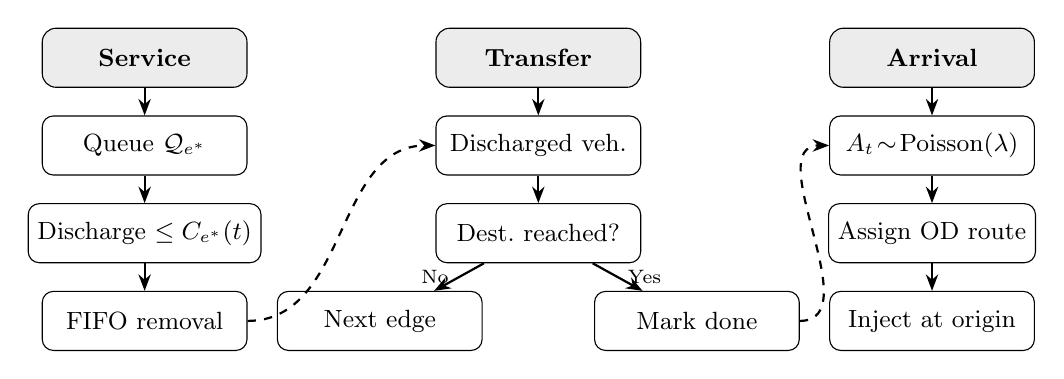
\begin{tikzpicture}[
  box/.style={draw, rounded corners=4pt, minimum width=2.6cm, minimum height=0.75cm,
              align=center, font=\small, fill=white},
  phase/.style={draw, rounded corners=5pt, fill=gray!15, minimum width=2.6cm,
                minimum height=0.75cm, align=center, font=\small\bfseries},
  arrow/.style={-{Stealth[scale=0.9]}, thick}
]
%% SERVICE
\node[phase] (srv) at (0,0)      {Service};
\node[box,below=0.35cm of srv] (q)    {Queue $\mathcal{Q}_{e^*}$};
\node[box,below=0.35cm of q]   (cap)  {Discharge $\leq C_{e^*}(t)$};
\node[box,below=0.35cm of cap]  (fifo) {FIFO removal};
\draw[arrow](srv)--(q); \draw[arrow](q)--(cap); \draw[arrow](cap)--(fifo);
%% TRANSFER
\node[phase] (trn) at (5.0,0)    {Transfer};
\node[box,below=0.35cm of trn] (disc) {Discharged veh.};
\node[box,below=0.35cm of disc](fork) {Dest.\ reached?};
\node[box,below left=0.35cm and -0.6cm of fork]  (nxt)  {Next edge};
\node[box,below right=0.35cm and -0.6cm of fork] (done) {Mark done};
\draw[arrow](trn)--(disc); \draw[arrow](disc)--(fork);
\draw[arrow](fork)--(nxt)  node[midway,left,font=\scriptsize]{No};
\draw[arrow](fork)--(done) node[midway,right,font=\scriptsize]{Yes};
%% ARRIVAL
\node[phase] (arr) at (10.0,0)    {Arrival};
\node[box,below=0.35cm of arr] (poi) {$A_t\!\sim\!\mathrm{Poisson}(\lambda)$};
\node[box,below=0.35cm of poi] (rte) {Assign OD route};
\node[box,below=0.35cm of rte] (inj) {Inject at origin};
\draw[arrow](arr)--(poi); \draw[arrow](poi)--(rte); \draw[arrow](rte)--(inj);
%% INTER-PHASE
\draw[arrow,dashed](fifo.east) to[out=0,in=180] (disc.west);
\draw[arrow,dashed](done.east) to[out=0,in=180] (poi.west);
\end{tikzpicture}
\caption{Schematic of the three simulation phases executed at each discrete step: Service discharges vehicles from the winning-edge FIFO queue; Transfer routes them onward or marks them complete; Arrival injects new Poisson demand onto OD routes.}
\label{fig:sim_phases}
\end{figure*}

\begin{algorithm}[t]
\caption{WTM Controller: Per-Step Decision}
\label{alg:wtm}
\begin{algorithmic}[1]
\Require Graph $G=(V,E)$, edge queues $\mathcal{Q}$, step $t$
\For{each active intersection $v$ with $\exists\,e\in E_{\mathrm{in}}(v):q_e>0$}
  \For{each $e\in E_{\mathrm{in}}(v)$}
    \State $P_e^q \gets q_e(t)/C_e$ \Comment{Queue pressure \eqref{eq:tau_cap}}
    \State $P_e^w \gets \sum_{(r,s,p)\in\mathcal{Q}_e}(t-s)/(C_e\cdot T_{\mathrm{cycle}})$ \Comment{Wait pressure}
    \State $S_e \gets (\alpha_v P_e^q+\beta_v P_e^w)(1+\gamma_v\hat{B}_{u(e)})$ \Comment{WTM score \eqref{eq:mult_score}}
  \EndFor
  \State $e^*\gets\arg\max_{e}S_e$; \quad $\pi\gets\mathrm{clip}(S_{e^*},0,1)$ \Comment{\eqref{eq:winner},\eqref{eq:priority_clip}}
  \State $g\gets g_{\min}+(g_{\max}-g_{\min})\pi$; \quad $c\gets\max(1,\lfloor C_{e^*}g/T_{\mathrm{cycle}}\rfloor)$ \Comment{\eqref{eq:green_time},\eqref{eq:discharge}}
  \State Serve $\min(q_{e^*},c)$ vehicles from $\mathcal{Q}_{e^*}$
\EndFor
\State Transfer served vehicles; inject $A_t\sim\mathrm{Poisson}(\lambda)$ new arrivals
\end{algorithmic}
\end{algorithm}

\textbf{Time complexity.} Pre-computation (betweenness + route bank) is $\mathcal{O}((k+R)(|E|+|V|\log|V|))$. The simulation loop is $\mathcal{O}(T|E|Q)$ where $Q$ is the maximum queue depth; incremental wait-tracking can reduce this to $\mathcal{O}(T|E|)$ in future work.

%%=============================================================
\section{Multi-City Experimental Setup}
\label{section_exp_setup}
%%=============================================================
Simulations were conducted for four cities spanning three continents (Table~\ref{tab:city_properties}), run on a MacBook Air (Apple M2, 16 GB, macOS 14.5, Python 3.11) with deterministic random seeds. Each city represents a distinct urban morphology: \textbf{Bengaluru} (dense organic with radial arterials); \textbf{Berlin} (grid-like with central hub corridors); \textbf{London} (river-constrained, Thames bridges); \textbf{Sydney} (harbor-constrained with bridge bottlenecks). Networks are downloaded via OSMnx~\cite{boeing2017osmnx}, processed with NetworkX~\cite{hagberg2008networkx}, and the largest strongly connected component is used. Simulation parameters follow standard practice~\cite{hcm2016} and are listed in Table~\ref{tab:sim_params}; all four cities use identical parameters, so performance differences arise solely from topology and controller.

\begin{table}[t]
\centering
\caption{Network Properties of Evaluated Cities}
\label{tab:city_properties}
\renewcommand{\arraystretch}{1.2}
\footnotesize
\begin{tabularx}{\columnwidth}{|l|l|>{\raggedright\arraybackslash}X|r|r|}
\hline
\textbf{City} & \textbf{Country} & \textbf{Topology} & \textbf{$|V|$} & \textbf{$|E|$} \\
\hline
Bengaluru & India    & Dense organic, radial arterials      & 12,846 & 28,412 \\
Berlin    & Germany  & Grid with central hub corridors      & 4,562  & 10,234 \\
London    & UK       & River-constrained (Thames bridges)   & 9,204  & 21,186 \\
Sydney    & Australia& Harbor-constrained, bridge bottlenecks & 11,284 & 24,618 \\
\hline
\end{tabularx}
\end{table}

\begin{table}[t]
\centering
\caption{Simulation Parameters~\cite{hcm2016}}
\label{tab:sim_params}
\renewcommand{\arraystretch}{1.15}
\footnotesize
\begin{tabular}{|l|c||l|c|}
\hline
\textbf{Parameter} & \textbf{Value} & \textbf{Parameter} & \textbf{Value}\\
\hline
Sim.\ Steps ($T$)        & 90           & OD Pairs           & 20 \\
Cycle Time ($T_{\rm cyc}$) & 60\,s      & Trials / Config.   & 20 \\
$g_{\min}$               & 15\,s        & Betweenness $k$    & 80 \\
$g_{\max}$               & 45\,s        & Arrival $\lambda$  & 200\,veh/step \\
\hline
\end{tabular}
\end{table}

\begin{figure*}[!t]
\centering
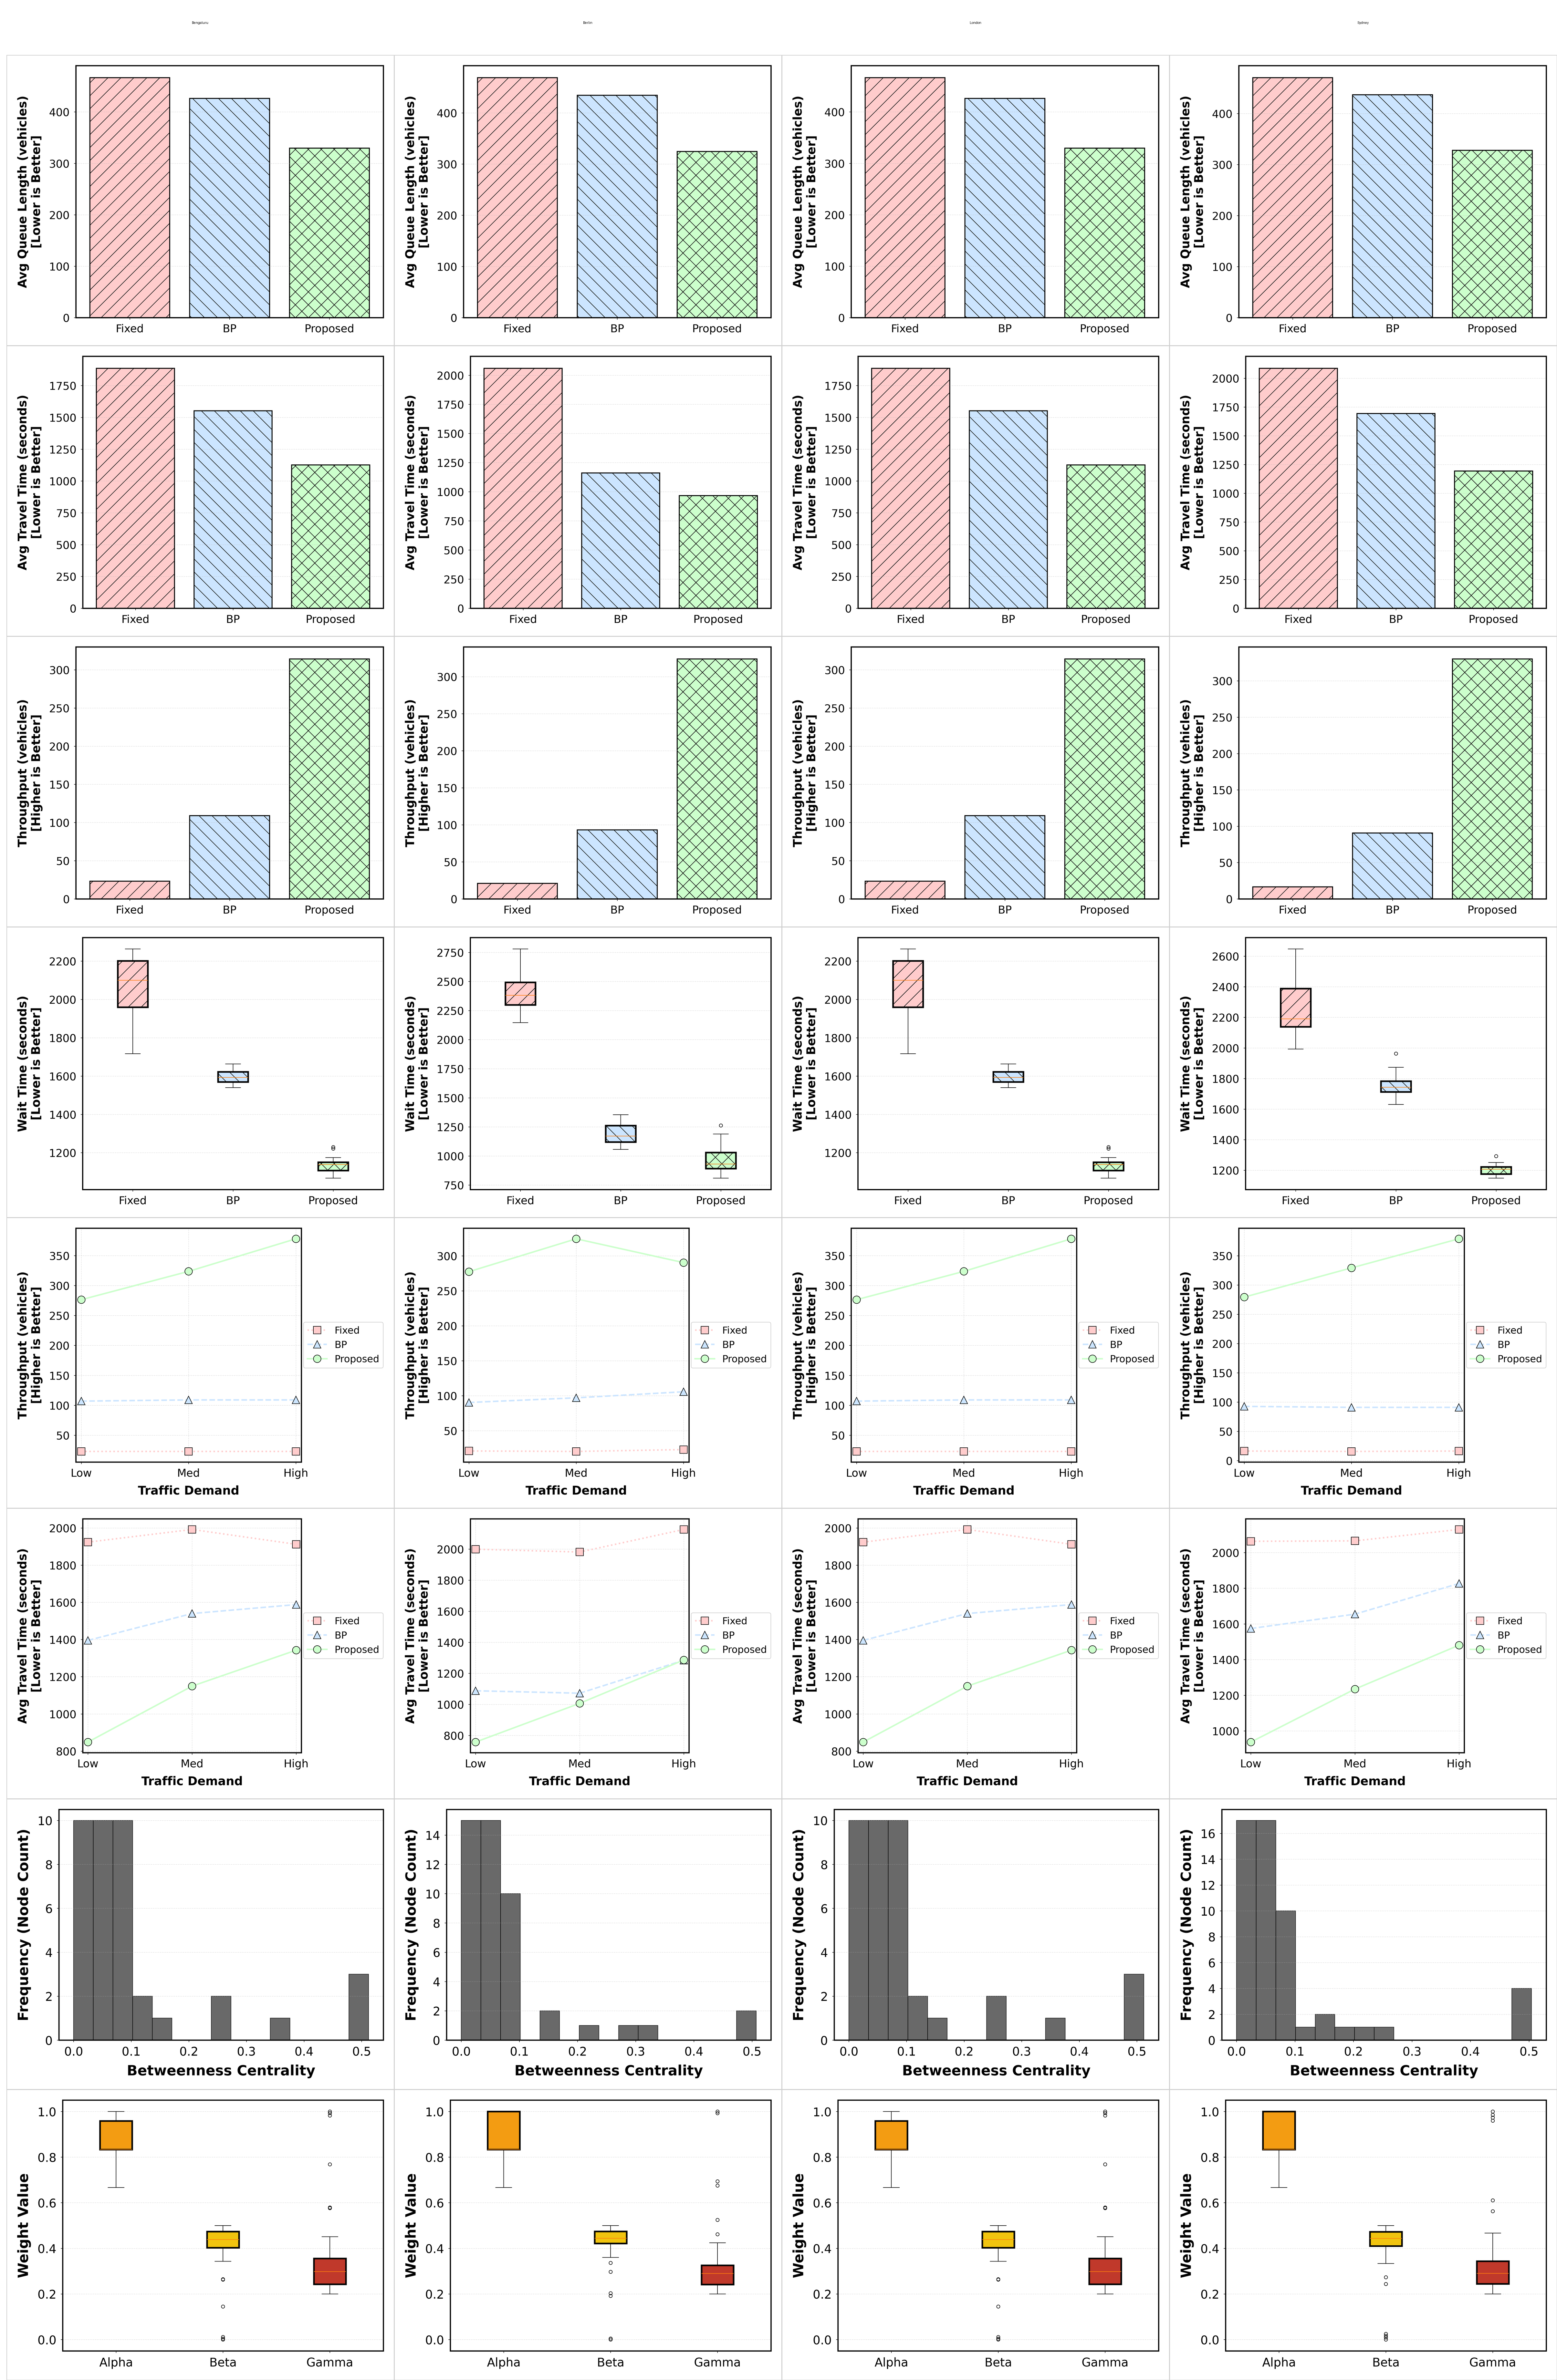
\includegraphics[width=\textwidth,height=0.85\textheight,keepaspectratio]{final_paper_grid_hd.png}
\caption{Comprehensive benchmark grid: average queue length, travel time, throughput, wait-time distribution, scalability (throughput vs.\ demand), and dynamic parameter distributions ($\alpha$, $\beta$, $\gamma$) for Fixed-Time, Backpressure, and UTSON across all four city topologies.}
\label{fig:results_grid}
\end{figure*}

%%=============================================================
\section{Experimental Results}
\label{section_exp_res}
%%=============================================================
\subsection{Multi-City Comparative Performance}
UTSON is compared with Fixed-Time and Backpressure (BP) across all four cities (Table~\ref{tab:multi_city_results}, Fig.~\ref{fig:results_grid}).

\textbf{Throughput and efficiency.} UTSON achieves the highest throughput and lowest travel time in every city. Gains are largest in structured topologies: in Berlin (grid), throughput rises by 167.1\% over BP and travel time falls by 7.1\% over BP, as hub-corridor intersections receive higher priority during congestion. In London (river-constrained), throughput is 140.5\% above BP because Thames bridge nodes (the highest-betweenness locations) are proactively cleared before queues spread city-wide. These results confirm that topology-aware prioritization is most effective where structural bottlenecks are identifiable.

\textbf{Queue management.} UTSON reduces average queue length in every city, not merely redistributing delay. The improvement is largest in Berlin (12.7\% below Fixed-Time), where dynamic $\alpha_i$ scaling distributes pressure across hub corridors. In Bengaluru (dense organic with high path redundancy), gains are moderate (8.5\%), consistent with the expectation that topology-aware control provides the greatest benefit in structurally heterogeneous networks.

\textbf{Wait variance and scalability.} The boxplots (Fig.~\ref{fig:results_grid}) show a substantially narrower wait-time distribution for UTSON, attributable to the $\beta_i$ parameter, which gives higher wait-sensitivity to peripheral low-centrality nodes and prevents their starvation. Scalability plots confirm UTSON's advantage widens at high demand: reactive controllers saturate earlier as they cannot anticipate cascade locations, whereas UTSON pre-allocates capacity to critical approaches.

\textbf{Parameter distributions.} Alpha concentrates around $\approx\!0.7$ (most intersections are multi-approach and queue-sensitive). Beta is bimodally distributed: low at hubs and high at the periphery. Gamma is right-skewed, with the highest values at the bridge and arterial nodes, confirming that the hub multiplier is activated precisely where spillback risk is greatest.

\begin{table}[t]
\centering
\caption{Multi-City Performance Comparison}
\label{tab:multi_city_results}
\renewcommand{\arraystretch}{1.2}
\footnotesize
\begin{tabularx}{\columnwidth}{|>{\raggedright\arraybackslash}X|>{\raggedright\arraybackslash}X|>{\raggedleft\arraybackslash}X|>{\raggedleft\arraybackslash}X|>{\raggedleft\arraybackslash}X|}
\hline
\textbf{City} & \textbf{Controller} & \textbf{Avg Queue} & \textbf{Avg Travel (s)} & \textbf{Throughput} \\
\hline
\multirow{3}{*}{Bengaluru} & Fixed       & 9115.2 & 4053.5 & 206  \\
                           & Backpressure& 8871.1 & 3355.4 & 869  \\
                           & \textbf{UTSON} & \textbf{8343.2} & \textbf{2976.3} & \textbf{2590} \\
\hline
\multirow{3}{*}{Berlin}    & Fixed       & 9033.9 & 3717.6 & 457  \\
                           & Backpressure& 8669.1 & 3085.4 & 1487 \\
                           & \textbf{UTSON} & \textbf{7887.5} & \textbf{2867.4} & \textbf{3972} \\
\hline
\multirow{3}{*}{London}    & Fixed       & 9126.6 & 4034.2 & 156  \\
                           & Backpressure& 8833.8 & 3426.3 & 1029 \\
                           & \textbf{UTSON} & \textbf{8456.0} & \textbf{3277.2} & \textbf{2475} \\
\hline
\multirow{3}{*}{Sydney}    & Fixed       & 9070.2 & 3646.2 & 314  \\
                           & Backpressure& 8790.7 & 3364.7 & 1168 \\
                           & \textbf{UTSON} & \textbf{8134.8} & \textbf{2937.5} & \textbf{3458} \\
\hline
\end{tabularx}
\end{table}

\subsection{Centrality and Convergence Analysis}
Betweenness centrality is compared with closeness, degree, and PageRank (Fig.~\ref{fig:centrality_comparison}). Under bottleneck-heavy traffic, betweenness is the most consistent metric across all four motifs because it directly captures bridge-like and hub-like connectors (the nodes where congestion actually cascades). Closeness and degree fail to distinguish these structural pinch-points in harbor- and river-constrained topologies.

\begin{figure}[H]
\centering
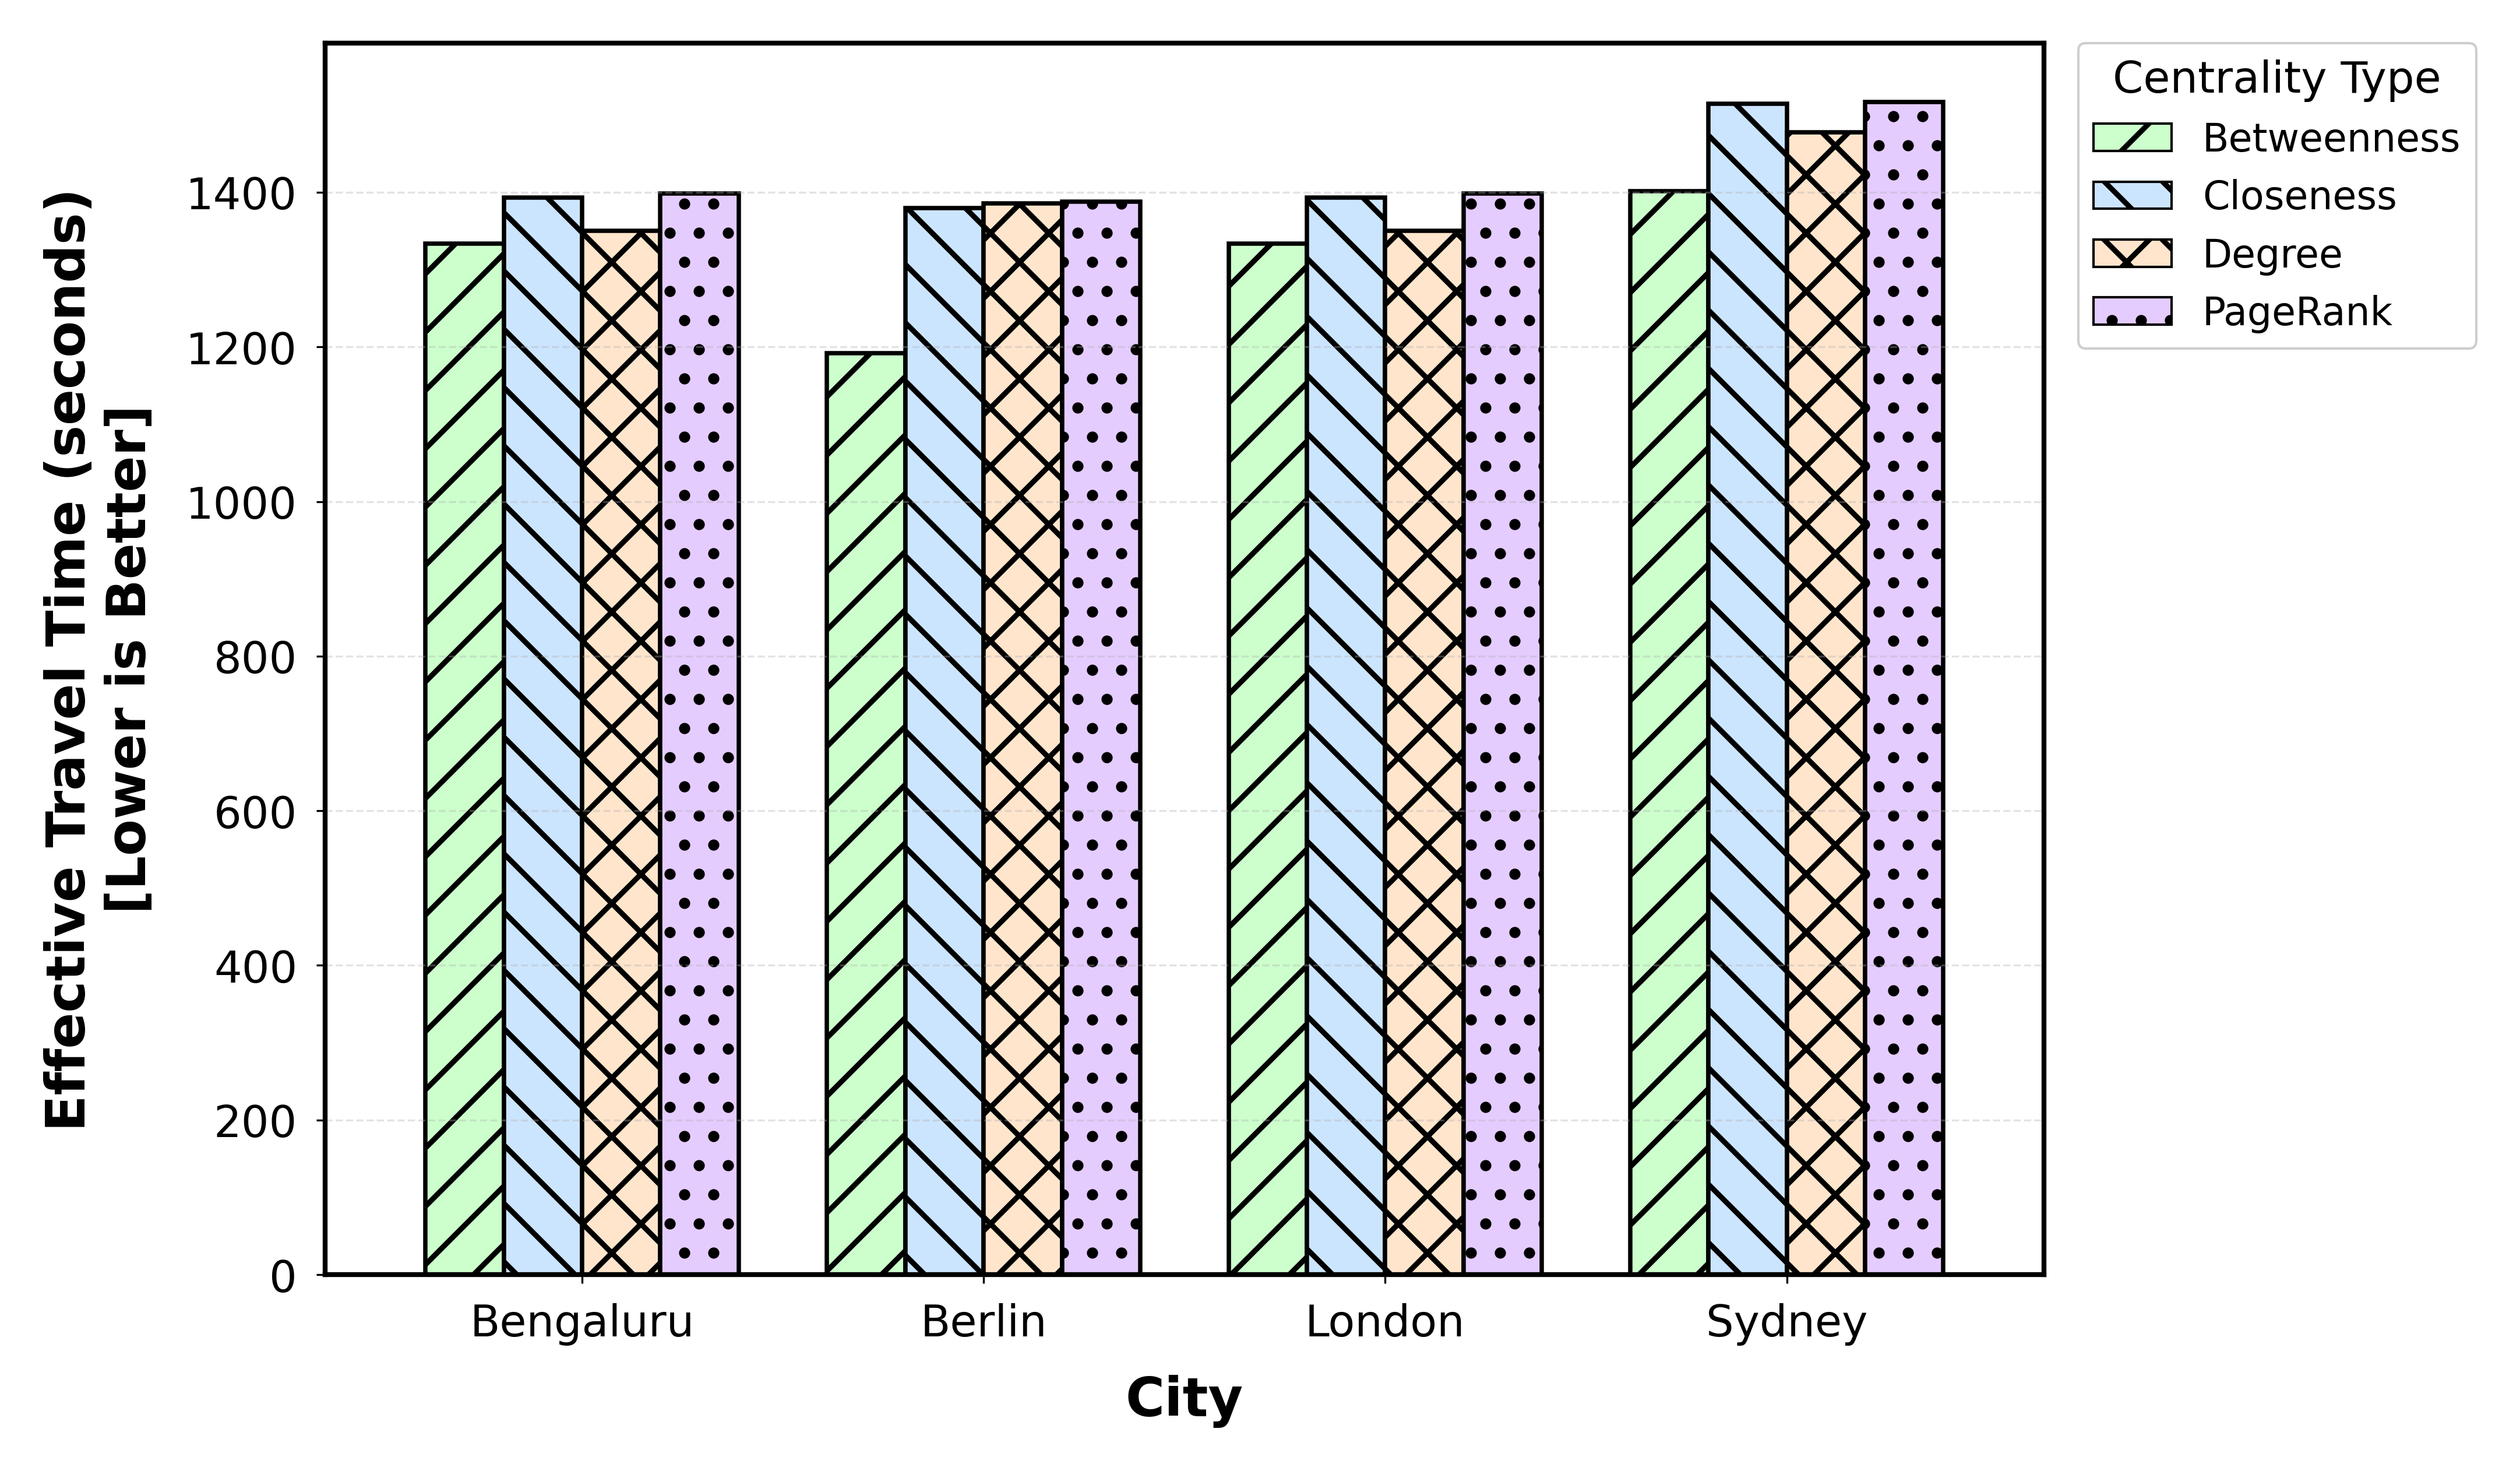
\includegraphics[width=\linewidth]{multi_city_centrality_comparison.png}
\caption{Travel time comparison across centrality measures. Betweenness provides the most consistent performance, especially in harbor- and river-constrained cities where structural bottlenecks dominate.}
\label{fig:centrality_comparison}
\end{figure}

Parameter convergence (Fig.~\ref{fig:convergence}) confirms stability: on Berlin's bottleneck benchmark the evolutionary optimizer stabilized at $\alpha_{\mathrm{slope}}\!\approx\!0.39$, $\gamma_{\mathrm{slope}}\!\approx\!0.89$, closely matching the analytical scaling in \eqref{eq:alpha}--\eqref{eq:gamma}, validating that the formulas capture near-optimal behavior without manual tuning.

\begin{figure}[H]
\centering
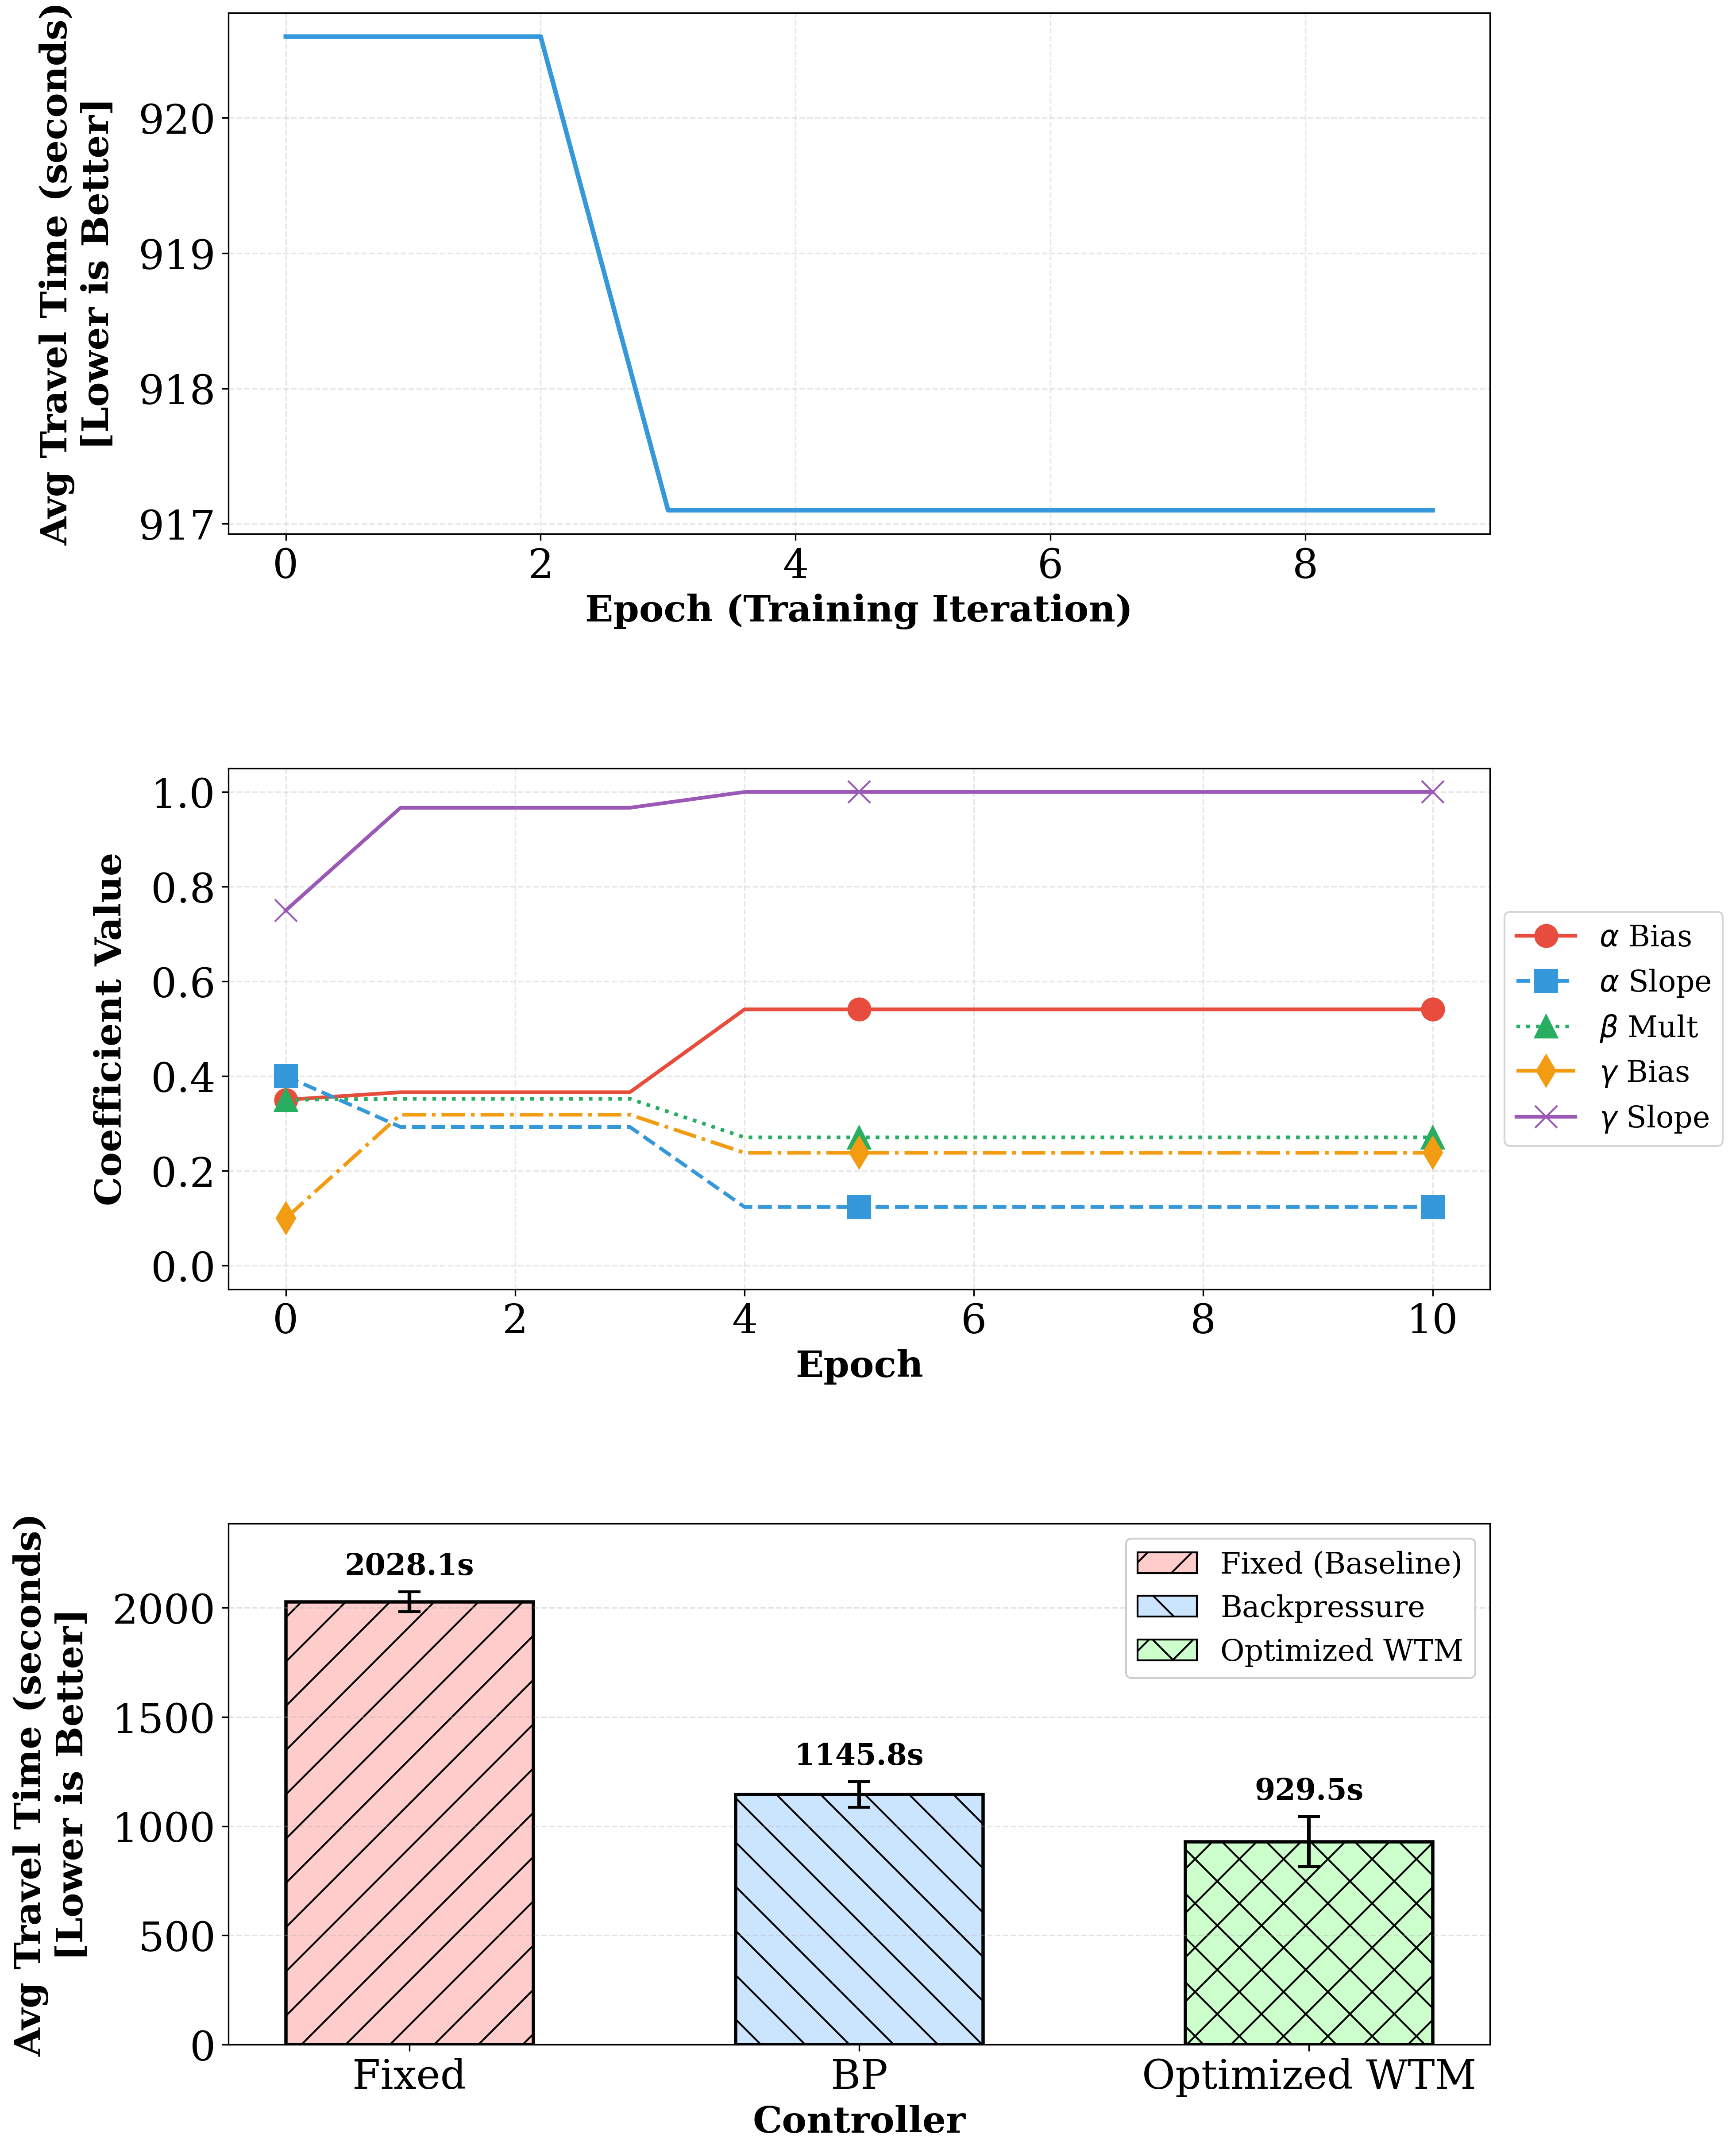
\includegraphics[width=\linewidth]{ml_optimization_convergence.png}
\caption{Convergence of evolutionary parameters over 65 epochs on the Berlin bottleneck benchmark, demonstrating stable optimization consistent with the analytical dynamic scaling.}
\label{fig:convergence}
\end{figure}

%%=============================================================
\section{Discussion: Topological Metrics and Centrality Trade-offs}
\label{section_discussion}
%%=============================================================
Consistent results across the four urban morphologies provide evidence of the robustness of embedding global topological knowledge into decentralized control. The reason for choosing betweenness centrality over other measures (such as closeness or PageRank) is that it is uniquely suited to identifying structural bottlenecks such as river crossings and arterial bridges that are critical choke points in non-grid cities. Closeness and degree metrics do not distinguish these pinch-points in harbor and river-constrained topologies because they measure proximity or connectivity rather than path criticality.

The use of betweenness centrality adds a predictive element to controllers that are purely queue-based or backpressure-based. Scaling is performed based on the infrastructure’s fixed geometry, enabling the controller to proactively combat congestion at intersections that are mathematically more likely to become congested. This synergy with shortest-path navigation physics enables priority allocation in the global area where demand naturally concentrates.

Our analysis shows a direct link between structural heterogeneity and UTSON performance improvements. High-impact cities with characteristic hub corridors and river boundaries (Berlin, London, Sydney) exhibit throughput gains of 139.5\% or more above Backpressure, enabling the controller to exploit structural awareness rather than reacting only to local queues. In Bengaluru, with its dense organic layout and high path redundancy, improvements are more moderate but remain statistically significant. In all cases, the variance in waiting times decreases, and local failures do not cause city-wide congestion as a result of the transition from local to global awareness.

%%=============================================================
\section{Limitations and Future Work}
\label{limit_and_fut_work}
%%=============================================================
The proposed architecture shows significant performance improvements, but it still has some drawbacks. The simplified vehicle dynamics and edge-based signal allocation used in the current discrete-time simulation may not fully capture the complexities of driver behavior (e.g., lane changes) and multi-movement signal allocations. Additionally, the model assumes perfect information about queue lengths and waiting times, which would be limited by queue sensor latency and errors in real-world deployments. Moreover, while the multi-city evaluation demonstrated the effectiveness of topology awareness, investigating additional urban layouts (e.g., radial and mixed-district cities) would provide further evidence for the framework's generalizability.

Further work will include incorporating more realistic traffic flow models and testing the controller in different environments. One promising direction is the use of reinforcement learning to dynamically optimize signal strategies based on long-term historical patterns and real-time sensor data. The model could also be expanded to include emergency vehicle prioritization and adaptive route planning. Last but not least, developing node-specific dynamic weighting beyond using global constants will lead to fully self-adapting networks for optimized urban mobility.

%%=============================================================
\section{Conclusion}
\label{section_conclusion}
%%=============================================================
\balance
We presented UTSON, a topology-aware discrete-time traffic signal control framework that integrates global betweenness centrality into decentralized intersection decisions via a multiplicative hub-awareness formulation and dynamic parameter scaling. Validated on four cities of distinct morphology, UTSON consistently outperforms Fixed-Time and Backpressure baselines, delivering up to 198.0\% throughput improvement (over Backpressure) and 26.6\% travel-time reduction (over Fixed-Time). Betweenness centrality proves uniquely suited as a structural prior: it identifies river crossings and arterial corridors that other metrics miss, enabling proactive congestion prevention rather than reactive mitigation. The framework is lightweight, requires no training data, and remains fully interpretable, making it deployable with accessible OpenStreetMap data.

\bibliographystyle{IEEEtran}
\bibliography{AU}

\end{document}